% ============================================================
% Monograph: Stochastic Calculus
% ============================================================
\documentclass[12pt,a4paper]{report}
\usepackage[utf8]{inputenc}
\usepackage[T1]{fontenc}
\usepackage[english]{babel}
\usepackage{lmodern,microtype}
\usepackage{amsmath,amssymb,amsthm,mathtools}
\usepackage{xcolor}
\usepackage{graphicx,float,booktabs,array}
\usepackage[colorlinks=true,linkcolor=blue!60!black,citecolor=green!50!black,urlcolor=blue]{hyperref}
\usepackage[backend=biber,style=alphabetic,sorting=nyt]{biblatex}
\addbibresource{references.bib}
\usepackage[top=2cm,bottom=2.5cm,left=2.5cm,right=2.5cm]{geometry}
\usepackage{fancyhdr}
\setlength{\headheight}{15pt}
\pagestyle{fancy}\fancyhf{}\fancyhead[R]{\thepage}\fancyhead[L]{\nouppercase{\leftmark}}
\renewcommand{\headrulewidth}{0.4pt}
\graphicspath{{./}{../}}
\theoremstyle{plain}
\newtheorem{theorem}{Theorem}[chapter]
\newtheorem{lemma}[theorem]{Lemma}
\theoremstyle{definition}
\newtheorem{definition}[theorem]{Definition}
\newtheorem{example}{Example}[chapter]
\newcommand{\R}{\mathbb{R}}
\newcommand{\E}{\mathbb{E}}
\newcommand{\F}{\mathcal{F}}
\newcommand{\dd}{\,\mathrm{d}}
\newcommand{\norm}[1]{\left\|#1\right\|}
\begin{document}

\begin{titlepage}\centering\vspace*{2cm}
{\Large University of Buenos Aires\par}\vspace{.5cm}
{\large Faculty of Exact and Natural Sciences\par}
{\large Stochastic Calculus\par}\vspace{3cm}
{\Huge\bfseries Diffusions and Score\par}\vspace{.3cm}
{\Large\bfseries The mathematics behind modern generative models\par}\vspace{2cm}
{\large Author: Gonzalo Josué Spina\par}\vfill{\large July 2026\par}
\end{titlepage}
\clearpage\tableofcontents\clearpage

\chapter{Introduction}\label{chap:introduction}
Diffusion models have recently become popular enough that short films and videos on social networks and streaming platforms can resemble Hollywood productions with very large budgets. This monograph presents, in an ordered and concise form, the principal results that lead to the equations explaining how these models work.

We can think of data---images, audio, or text gathered from different sources or generated by a camera---as realizations of an unknown underlying distribution. If we can estimate that distribution well, we can generate arbitrarily many distinct samples with the same statistical structure.

The method starts from a data set whose samples represent an unknown population distribution. It progressively adds noise through a stochastic differential equation, obtains a new distribution at a final time $T$, and then follows the reverse path to estimate the original distribution. This noise injection is not ad hoc: recovering the original distribution requires estimating how its density evolves in time, which in turn makes it possible to construct the reverse dynamics.

\chapter{Diffusion processes}\label{chap:diffusion}
Within the theory of stochastic differential equations, a diffusion is a stochastic process $X_t=X(t,\omega)$ that satisfies an Itô stochastic differential equation (SDE)
\begin{equation}\dd X_t=u(t,X_t)\dd t+\sigma(t,X_t)\dd B_t,\qquad X_0=Z,\label{eq:sde}\end{equation}
where $u:[0,T]\times\R^d\to\R^d$ determines the deterministic evolution, $\sigma:[0,T]\times\R^d\to\R^{d\times m}$ determines the intensity and direction of the noise, and $B_t$ is an $m$-dimensional Brownian motion with respect to a filtration $(\F_t)_{t\geq0}$. The solution $X_t$ must itself be adapted to that filtration. Equivalently, \eqref{eq:sde} is understood in integral form as
\begin{equation}X_t=Z+\int_0^t u(s,X_s)\dd s+\int_0^t\sigma(s,X_s)\dd B_s.\label{eq:sde-integral}\end{equation}
The coefficient $u$ is the \emph{drift}; it describes the local deterministic tendency. The diffusion coefficient $\sigma$ specifies how Brownian noise acts on the process.

\begin{theorem}[Existence and uniqueness]\label{thm:existence}
Let $u$ and $\sigma$ be measurable functions for which there are constants $C,D>0$ such that, for every $t\in[0,T]$ and $x,y\in\R^d$,
\begin{equation}\norm{u(t,x)-u(t,y)}+\norm{\sigma(t,x)-\sigma(t,y)}\leq C\norm{x-y},\label{eq:lipschitz}\end{equation}
and
\begin{equation}\norm{u(t,x)}^2+\norm{\sigma(t,x)}^2\leq D(1+\norm{x}^2).\label{eq:growth}\end{equation}
If $Z$ is $\F_0$-measurable and $\E[\norm Z^2]<\infty$, the SDE \eqref{eq:sde} admits a unique continuous strong solution on $[0,T]$.
\end{theorem}
Condition \eqref{eq:lipschitz} is global Lipschitz continuity and guarantees uniqueness. The linear-growth condition \eqref{eq:growth} prevents finite-time explosion. Although the solution is not always available in closed form, it can be approximated numerically.

\begin{example}[Ornstein--Uhlenbeck process]\label{ex:ou}
The Ornstein--Uhlenbeck (OU) process is the diffusion on $\R$
\begin{equation}\dd X_t=-X_t\dd t+\sigma\dd B_t,\qquad X_0=x_0,\label{eq:ou}\end{equation}
with $\sigma>0$. Its coefficients are globally Lipschitz and have linear growth, so Theorem~\ref{thm:existence} applies. Variation of constants gives
\[X_t=x_0e^{-t}+\sigma\int_0^t e^{-(t-s)}\dd B_s.\]
By the properties of the Itô integral, $X_t\mid X_0=x_0$ is Gaussian with
\[\E^{x_0}[X_t]=x_0e^{-t},\qquad \mathrm{Var}(X_t\mid X_0=x_0)=\frac{\sigma^2}{2}(1-e^{-2t}).\]
As $t\to\infty$, its mean tends to $0$ and its variance to $\sigma^2/2$, independently of $x_0$. Thus the law of $X_t$ converges to $\mathcal N(0,\sigma^2/2)$.
\begin{figure}[H]\centering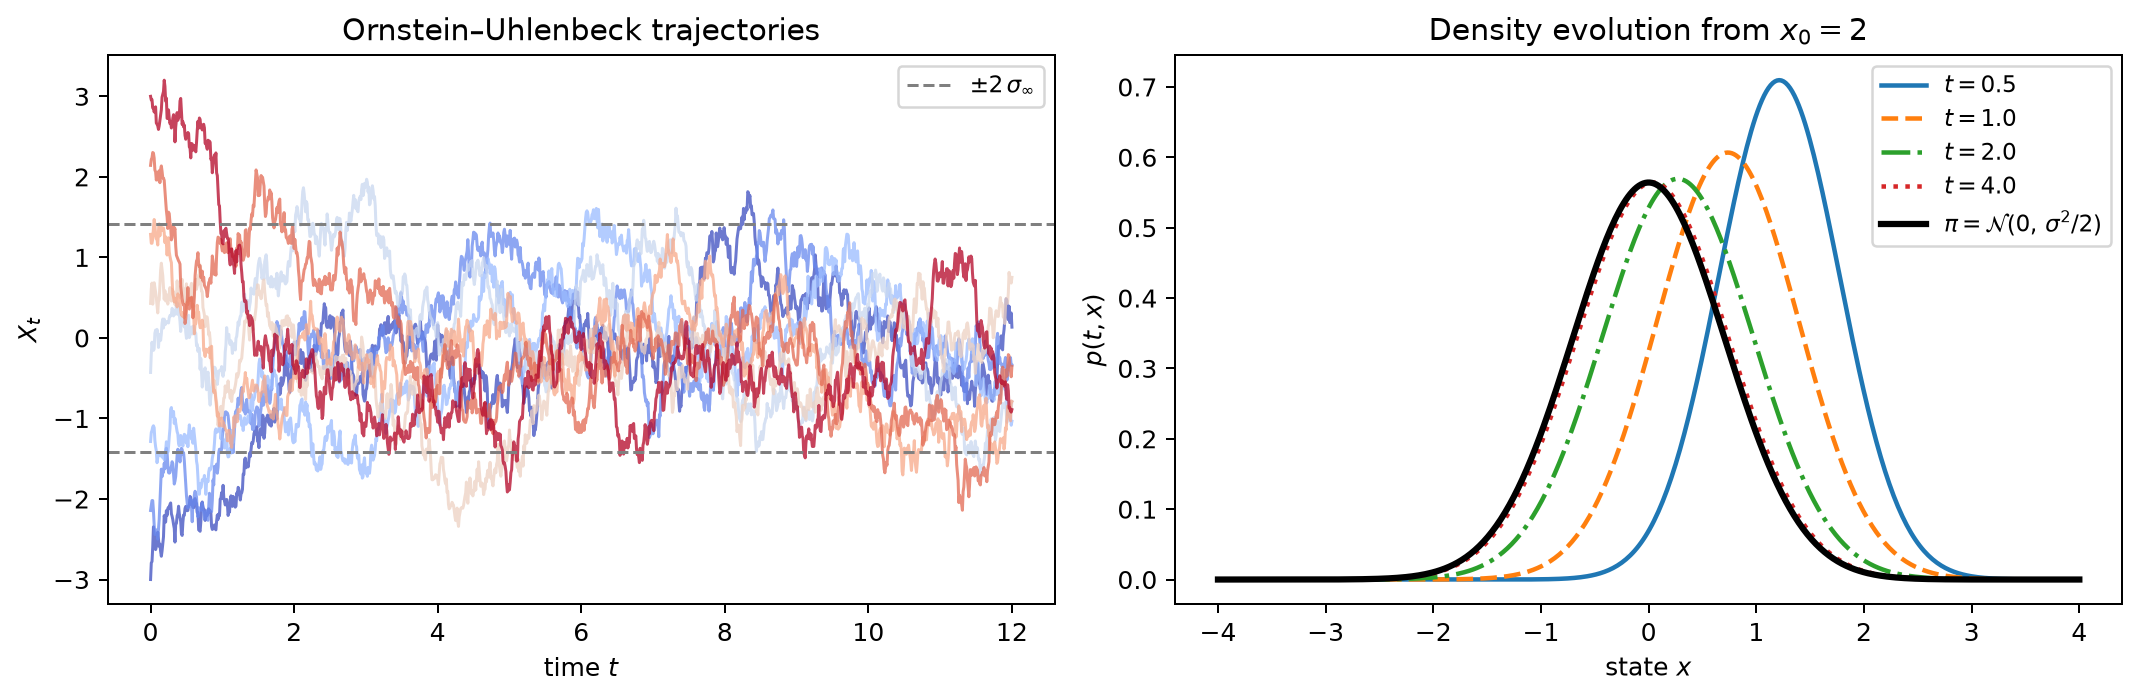
\includegraphics[width=\textwidth]{ou_trajectories_en.png}
\caption{Left: OU trajectories with $\sigma=1$ from different initial states $x_0\in[-3,3]$. Dashed lines mark the band $\pm2\sigma_\infty$ of the stationary distribution. Right: $p(t,\cdot)$ from $x_0=2$ at several times; the black curve is $\pi=\mathcal N(0,\sigma^2/2)$.}\label{fig:ou}\end{figure}
\end{example}

\chapter{Density evolution}\label{chap:density}
The density $p_t(x)=p(t,x)$ of a diffusion contains all information about its distribution at time $t$. We now derive the partial differential equation that governs that density. The route is through the infinitesimal generator, which describes the rate of change in the expectation of an observable, and the Kolmogorov equations.

\begin{definition}[Infinitesimal generator]\label{def:generator}
For a Markov diffusion $(X_t)_{t\geq0}$, its infinitesimal generator is the linear differential operator
\[\mathcal A_t f(x)=\lim_{h\downarrow0}\frac{\E^x[f(X_{t+h})]-f(x)}{h},\]
for functions $f$ for which the limit exists.
\end{definition}
It is the analogue of a derivative in ordinary calculus: it measures the instantaneous change of the expected observable $f(X_t)$.

\begin{lemma}[Itô formula in expectation]\label{lem:ito}
Let $X_t=x+\int_0^t u(s,\omega)\dd s+\int_0^t v(s,\omega)\dd B_s$, with $X_0=x$, and let $f\in C^2(\R^d)$ have compact support. Under the usual boundedness assumptions,
\[\E^x[f(X_t)]=f(x)+\E^x\!\left[\int_0^t\left(u_i\partial_i f(X_s)+\frac12(vv^\top)_{ij}\partial_{ij}f(X_s)\right)\dd s\right].\]
\end{lemma}
\begin{theorem}[Generator of a diffusion]\label{thm:generator}
If $X_t$ satisfies \eqref{eq:sde} and $f\in C_0^2(\R^d)$, then
\begin{equation}\mathcal A_t f(x)=u_i(t,x)\partial_i f(x)+\frac12(\sigma\sigma^\top)_{ij}(t,x)\partial_{ij}f(x).\label{eq:generator}\end{equation}
\end{theorem}
Combining Lemma~\ref{lem:ito} and Theorem~\ref{thm:generator} yields the stochastic counterpart of the fundamental theorem of calculus.
\begin{theorem}[Dynkin's formula]\label{thm:dynkin}
For $f\in C^2(\R^d)$,
\begin{equation}\E^x[f(X_t)]=f(x)+\E^x\!\left[\int_0^t\mathcal A_s f(X_s)\dd s\right].\label{eq:dynkin}\end{equation}
\end{theorem}
Dynkin's formula also provides the two Kolmogorov equations. The backward equation describes the expectation of a future observable conditional on the current state.
\begin{theorem}[Backward Kolmogorov equation]\label{thm:backward}
Let $X_t$ satisfy \eqref{eq:sde}, $T>0$, and $f\in C_b^2(\R^d)$. If $u^i$ and $a^{ij}=(\sigma\sigma^\top)^{ij}$ are Hölder continuous and $a$ is uniformly elliptic, then $v(t,x)=\E^x[f(X_T)]$ is the unique classical solution of
\[\frac{\partial v}{\partial t}(t,x)+\mathcal A_t v(t,x)=0,\qquad v(T,x)=f(x).\]
\end{theorem}
To obtain the equation for $p$, write Dynkin's formula against the density and differentiate:
\[\int_{\R^d}f(x)\,\partial_t p(t,x)\dd x=\int_{\R^d}(\mathcal A_t f)(x)p(t,x)\dd x.\]
Define the adjoint $\mathcal A_t^*$ by $\int(\mathcal A_t f)p=\int f(\mathcal A_t^*p)$. Since this identity holds for all compactly supported smooth $f$, the density satisfies the following result.
\begin{theorem}[Fokker--Planck equation]\label{thm:fp}
Under the regularity and ellipticity hypotheses of Theorem~\ref{thm:backward}, a density $p$ evolves according to $\partial_t p=\mathcal A_t^*p$, or explicitly
\begin{equation}\frac{\partial p}{\partial t}=-\partial_i[u_i(t,x)p(t,x)]+\frac12\partial_{ij}\left[(\sigma\sigma^\top)_{ij}(t,x)p(t,x)\right].\label{eq:fp}\end{equation}
\end{theorem}
\begin{example}[Fokker--Planck equation for OU]\label{ex:fp-ou}
For \eqref{eq:ou}, $u(t,x)=-x$ and $a(t,x)=\sigma^2$, so
\[\frac{\partial p}{\partial t}=\frac{\partial}{\partial x}(xp)+\frac{\sigma^2}{2}\frac{\partial^2p}{\partial x^2}.\]
The density of $\mathcal N(0,\sigma^2/2)$ satisfies $\mathcal A^*p_\infty=0$; it is the stationary distribution found directly in Example~\ref{ex:ou}.
\end{example}

\chapter{Reverse-time diffusion}\label{chap:reverse}
So far we have followed a diffusion forward from its initial distribution. We now want the opposite path: starting from its distribution at $T>0$, construct a process that runs backward and recovers the distribution at time zero. The key result is that this reverse process is itself a diffusion.

Define the time-reversed process by $\hat X_t=X_{T-t}$, $t\in[0,T]$. The non-trivial part is constructing a Brownian motion adapted to the decreasing filtration. Anderson~\cite{Anderson1982} proves that this construction yields the following reverse SDE.
\begin{theorem}[Time reversal, Anderson]\label{thm:reverse}
Suppose $u$ and $\sigma$ satisfy Theorem~\ref{thm:existence}, and that $X_t$ has a strictly positive density $p\in C^{1,2}([0,T]\times\R^d)$ satisfying \eqref{eq:fp}. Let $a=\sigma\sigma^\top$. Then there is a Brownian motion $\hat B_t$ for which $\hat X_t$ is a Markov diffusion satisfying
\begin{equation}\dd\hat X_t=\hat u(t,\hat X_t)\dd t+\hat\sigma(t,\hat X_t)\dd\hat B_t,\label{eq:reverse-sde}\end{equation}
where
\begin{align}\hat u^{\,i}(t,x)&=-u^i(T-t,x)+\frac{1}{p(T-t,x)}\partial_j\left[a^{ij}(T-t,x)p(T-t,x)\right],\label{eq:reverse-drift}\\
\hat\sigma(t,x)&=\sigma(T-t,x).\nonumber\end{align}
\end{theorem}
\begin{proof}[Proof sketch]
For $f\in C_0^2(\R^d)$, Bayes' rule expresses $\E[f(X_{T-t-h})\mid X_{T-t}=x]$ using the forward transition density and $p_{T-t-h}$. Differentiating in $h$, the backward Kolmogorov equation differentiates the transition density and Fokker--Planck differentiates $p_{T-t-h}$. Moving the generator by $L^2$ duality and taking $h\downarrow0$ yields
\[\hat{\mathcal A}_t f(x)=\frac12a^{ij}(T-t,x)\partial_{ij}f(x)+\hat u^{\,i}(t,x)\partial_i f(x),\]
with the drift in \eqref{eq:reverse-drift}.

For the driving noise, Anderson defines an auxiliary process $\tilde B_t$ by
\[\dd\tilde B_t^k=\dd B_t^k+\frac{1}{p(t,X_t)}\partial_j[p(t,X_t)\sigma^{jk}(t,X_t)]\dd t.\]
The joint Fokker--Planck equation shows that the density of $(X_t,\tilde B_t)$ factorizes as $p(t,x)\phi(\beta,t)$, where $\phi$ is a Gaussian heat kernel. Thus the relevant increments of $\tilde B$ are independent of the future state and Gaussian. Reparameterizing time with $\tau=T-t$ and setting $\hat B_\tau=\tilde B_T-\tilde B_{T-\tau}$ supplies the Brownian motion in \eqref{eq:reverse-sde}.
\end{proof}

\chapter{Score and score-based generation}\label{chap:score}
Song et al.~\cite{Song2021} give a unified framework for data generation based on the preceding machinery. Given samples from an unknown distribution $p_0$, a forward SDE gradually turns $p_0$ into a known distribution $p_T$, usually a Gaussian prior. By Theorem~\ref{thm:reverse}, a diffusion can travel in the opposite direction from $p_T$ back to $p_0$. Its drift depends on the gradient of the log density, called the \emph{score}. If we learn that score for every $t\in[0,T]$, we can simulate the reverse process and generate new samples from $p_0$.

\paragraph{Ergodicity and convergence to the prior.}
The forward process must produce a distribution that can be sampled at the start of the reverse process. If it is \emph{ergodic}---it forgets its initial condition and converges to a unique stationary distribution $\pi$---then, for sufficiently large $T$, $p_T\approx\pi$ independently of $p_0$. We can therefore sample $\pi$ directly. The OU process has this property, with $\pi=\mathcal N(0,\sigma^2/2)$.

\paragraph{The score and its role in reverse diffusion.}
\begin{definition}[Score]\label{def:score}For a diffusion $X_t$ with density $p(t,x)$, the score is $s(t,x)=\nabla_x\log p(t,x)$.\end{definition}
If $\sigma=\sigma(t)$ depends only on time, the spatial derivatives of $a$ vanish. The reverse drift simplifies to
\[\hat u(t,x)=-u(T-t,x)+\sigma(T-t)^2\nabla_x\log p(T-t,x),\]
and the reverse SDE is
\begin{equation}\dd\hat X_t=\left[-u(T-t,\hat X_t)+\sigma(T-t)^2\nabla_x\log p(T-t,\hat X_t)\right]\dd t+\sigma(T-t)\dd\hat B_t.\label{eq:reverse-score}\end{equation}
The score is the only unavailable ingredient: $u$ and $\sigma$ are chosen as part of the forward process, whereas $\nabla_x\log p(t,x)$ depends on the unknown $p_0$ through density evolution.
\begin{figure}[H]\centering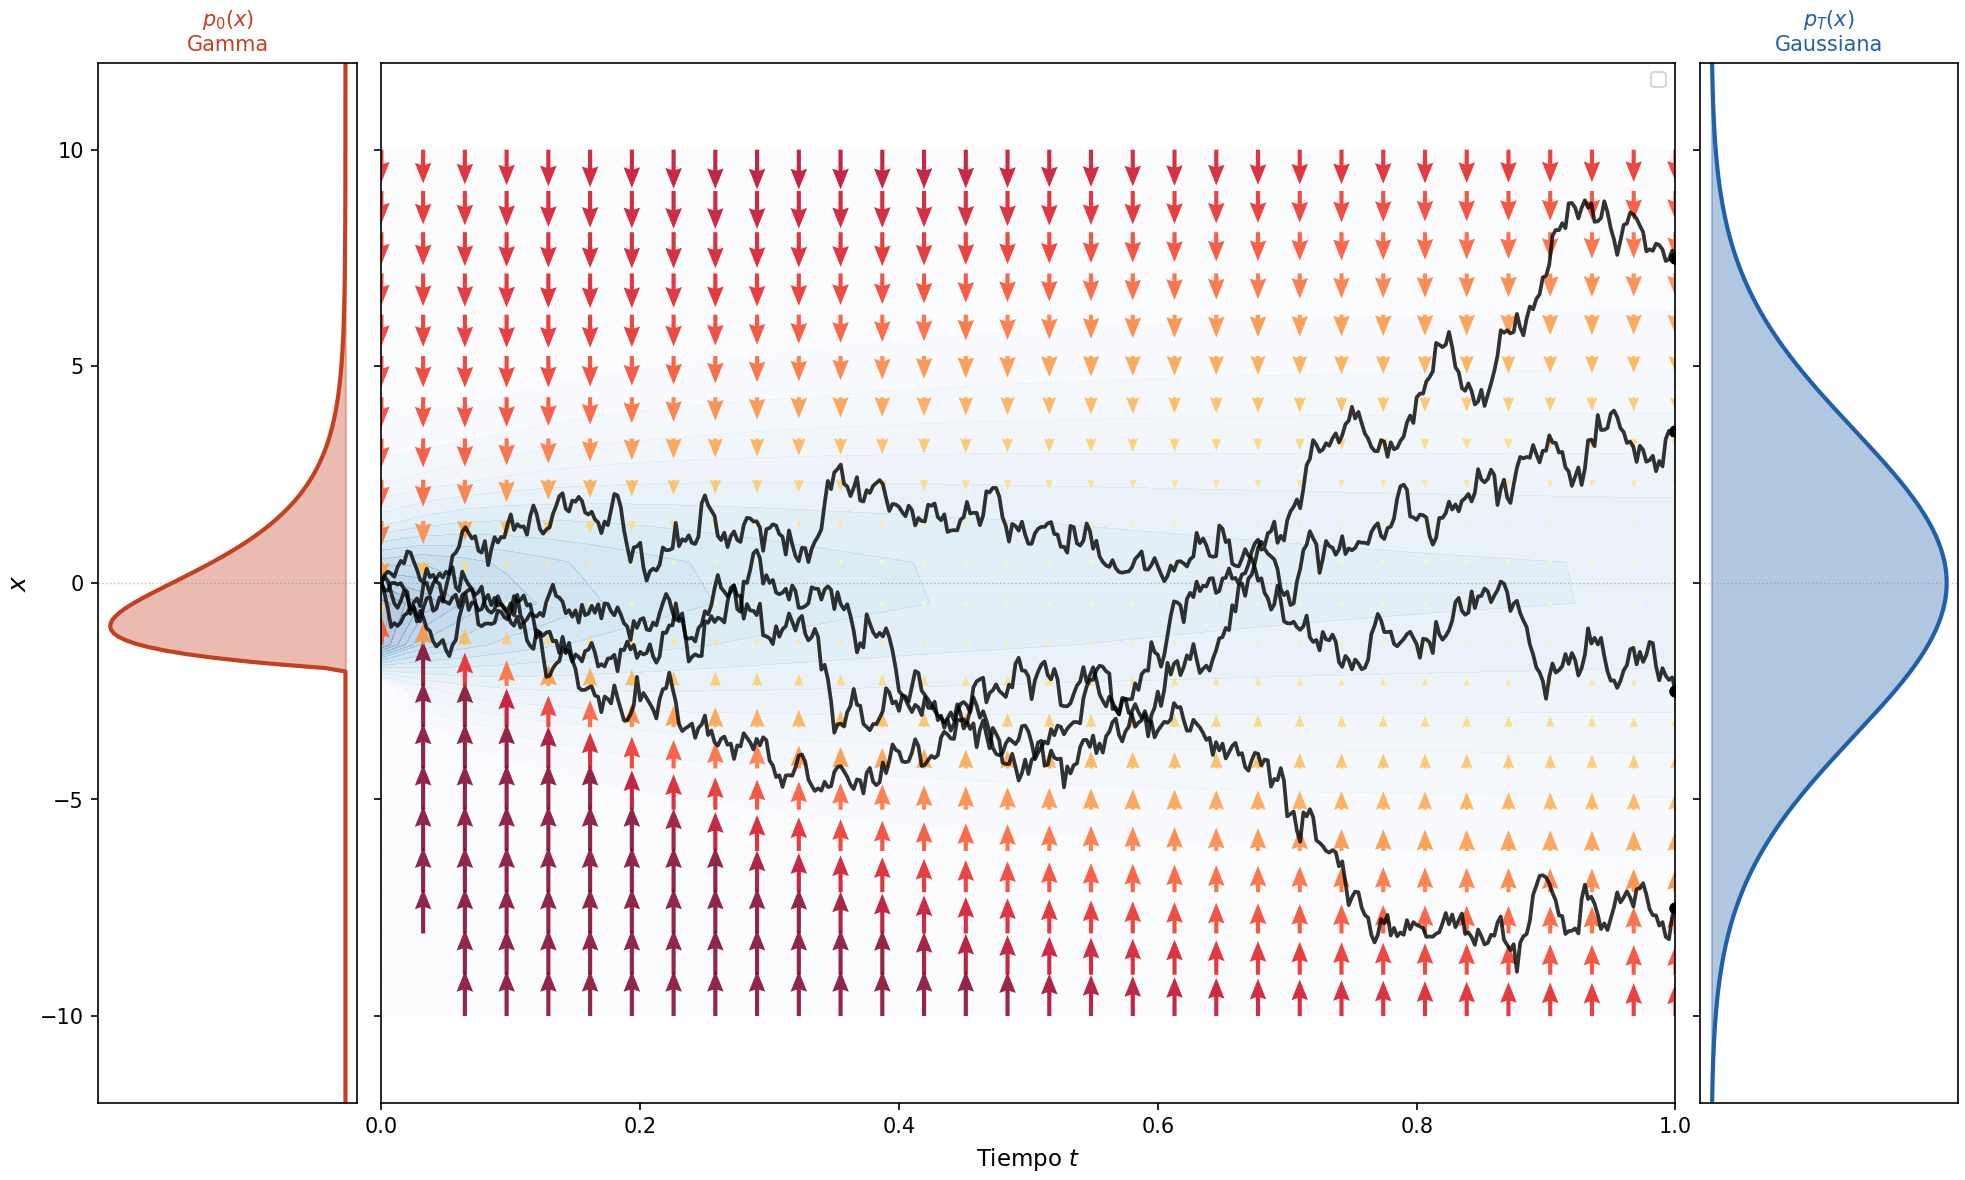
\includegraphics[width=\textwidth]{fig2_score.png}
\caption{The score field along the forward path. Arrows point toward higher-density regions. The figure can be read left to right as diffusion or right to left as reverse guidance.}\label{fig:score}\end{figure}

\begin{example}[Score and reverse diffusion for OU]\label{ex:score-ou}
For OU, \eqref{eq:reverse-score} becomes
\[\dd\hat X_t=\left[\hat X_t+\sigma^2\nabla_x\log p(T-t,\hat X_t)\right]\dd t+\sigma\dd\hat B_t,\]
with $\hat X_0\sim\mathcal N(0,\sigma^2/2)$. The drift changes sign relative to the forward process ($-x\mapsto+x$): the forward dynamics pull toward zero, while the reverse dynamics move away and the score corrects the path to recover the shape of $p_0$.

The marginal density is $p(t,x)=\int p_{X_t\mid X_0=x_0}(x)p_0(x_0)\dd x_0$. For OU this is a Gaussian mixture with conditional mean $x_0e^{-t}$ and variance $\frac{\sigma^2}{2}(1-e^{-2t})$. It depends on unknown $p_0$, so the marginal score is not directly available. The conditional score, however, is analytic:
\[\nabla_x\log p_{X_t\mid X_0=x_0}(x)=-\frac{x-x_0e^{-t}}{\frac{\sigma^2}{2}(1-e^{-2t})}.\]
The network $s_\theta(t,x_t)$ is trained on forward-generated pairs $(x_0,x_t)$ to predict this conditional score, and it is then used as an approximation to the marginal score in the reverse SDE.
\end{example}

\paragraph{Learning the score: denoising score matching.}
The formal bridge between marginal and conditional scores is obtained by differentiating the marginal density under the integral and applying Bayes' rule~\cite{Hyvarinen2005}:
\[\nabla_x\log p(t,x)=\int\nabla_x\log p_{X_t\mid X_0=x_0}(x)\,p_{X_0\mid X_t=x}(x_0)\dd x_0.\]
Conditioned on $X_t=x$, the marginal score is the posterior average of the conditional score. Vincent~\cite{Vincent2011} and Song et al.~\cite{Song2021} show that the minimizer of the inaccessible squared error to the marginal score is also the minimizer of the computable denoising objective
\begin{equation}\tilde J(\theta)=\int_0^T\lambda(t)\,\E_{p_0(x_0)p(x_t\mid x_0)}\!\left[\norm{s_\theta(t,x_t)-\nabla_{x_t}\log p_{X_t\mid X_0=x_0}(x_t)}^2\right]\dd t.\label{eq:dsm}\end{equation}
The expectation is over $x_0\sim p_0$ and $x_t\mid x_0$ simulated by the forward process. In practice, a neural network is optimized over a discrete set of noise times.

\paragraph{Generation algorithm.}
With $s_\theta$ trained, substitute it into \eqref{eq:reverse-score} and integrate with Euler--Maruyama~\cite{Oksendal2003}, using $\Delta t=T/N$:
\begin{enumerate}
\item Sample $x_T\sim\pi=\mathcal N(0,\sigma^2/2)$.
\item For $k=N,N-1,\ldots,1$, set $t_k=k\Delta t$, sample $z_k\sim\mathcal N(0,I)$, and update
\[x_{t_{k-1}}=x_{t_k}+\left[-u(t_k,x_{t_k})+\sigma(t_k)^2s_\theta(t_k,x_{t_k})\right]\Delta t+\sigma(t_k)\sqrt{\Delta t}\,z_k.\]
\item Return $x_0$ as an approximate sample from $p_0$.
\end{enumerate}

\paragraph{Numerical experiment.}
To illustrate the construction, we choose $p_0$ to be a Gamma distribution shifted to have mean zero, construct an OU forward process with $\sigma=1$ and $T=5$, and learn its score with a neural network trained by denoising score matching. Figure~\ref{fig:histogram} shows that the generated samples reproduce the original distribution in this one-dimensional example (Kolmogorov--Smirnov test: $p=0.69$).
\begin{figure}[H]\centering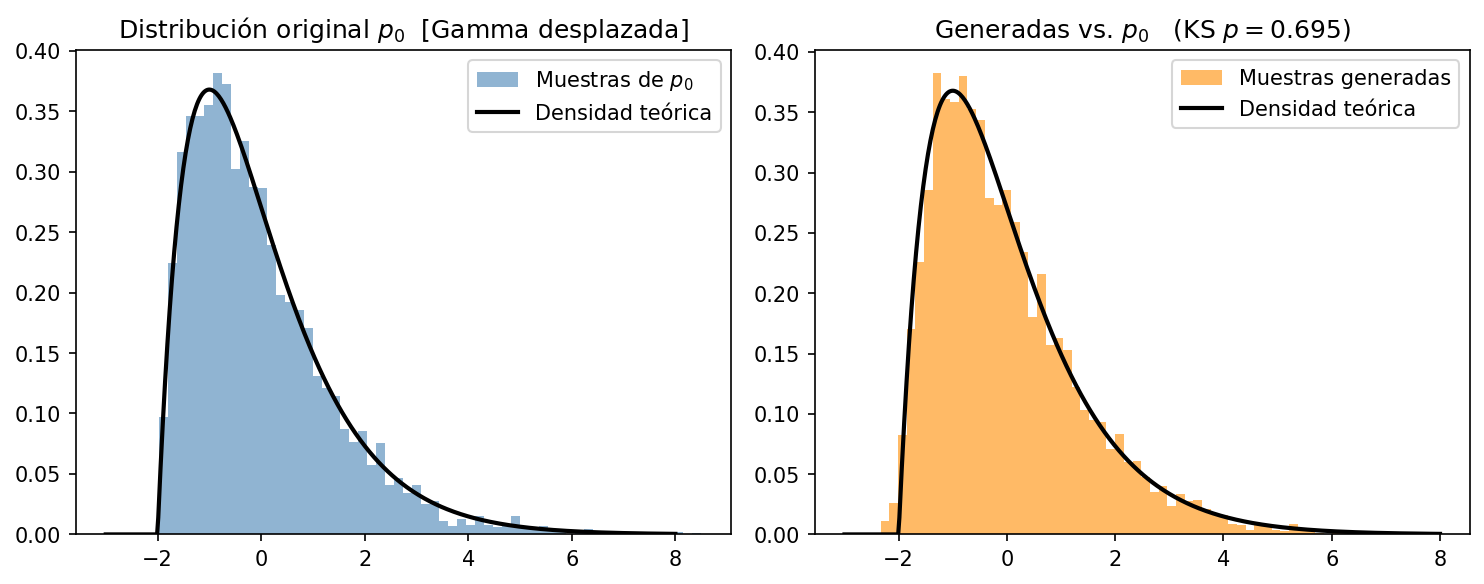
\includegraphics[width=\textwidth]{score_matching_demo.png}
\caption{Left: reference samples from $p_0$ (shifted Gamma) and its theoretical density. Right: samples generated by the reverse process overlaid on the same density.}\label{fig:histogram}\end{figure}

\printbibliography[heading=bibintoc,title={References}]
\end{document}
